\chapter{进阶感知：理解随时间积累的误差}
\begin{notebox}
\textbf{目标}\quad 区分白噪声与持久偏置，推导随机游走的步长与方差，用独立重复试验检查模型。\\
\textbf{实验}\quad 单轴偏置工具可独立运行；后半部分提供延迟、逐束畸变与复杂环境的扩展练习。
\end{notebox}
\section{每次重新抽样，与保留上一次状态}
第 06 章每采样白噪声 $n_k$ 相互独立、均值为零、标准差为 $\sigma_n$。
若静止陀螺仪还带有缓慢变化的偏置 $b_k$，测量写为
\[
 y_k=y_k^{\rm ideal}+b_k+n_k.
\]
白噪声在下一次采样重新抽取；偏置则作为状态保存，在旧值上加一个小增量。
即使真实角速度为零，测量也可能在一段时间内持续偏向同一侧。
本附录使用最简单的零均值独立增量来模拟这种缓慢漂移：
\[
 b_{k+1}=b_k+\eta_k.
\]
先确定增量的方差如何随时间变化，再写代码生成它。

\section{为什么增量要乘时间间隔的平方根}
设 $b_0$ 已知，要求同样经过 $T$ 秒后，偏置分散程度与数值采样频率无关。
以 $\Delta t$ 为步长，共有 $K=T/\Delta t$ 个独立增量。
若每步方差为 $q(\Delta t)$，则
\[
 \operatorname{Var}(b_K-b_0)
 =\operatorname{Var}\left(\sum_{k=0}^{K-1}\eta_k\right)=Kq(\Delta t).
\]
希望总方差按 $\sigma_b^2T$ 增长，就应令
$Kq=\sigma_b^2T$，从而 $q(\Delta t)=\sigma_b^2\Delta t$。
标准正态样本 $\xi_k$ 的方差为 1，乘以一个数会让方差乘该数的平方，因此
\begin{equation}
 \eta_k=\sigma_b\sqrt{\Delta t}\,\xi_k,\qquad
 \xi_k\sim\mathcal N(0,1),\qquad
 b_{k+1}=b_k+\sigma_b\sqrt{\Delta t}\,\xi_k.
 \label{eq:bias_step}
\end{equation}
陀螺偏置 $b$ 单位为 rad/s；$\sigma_b$ 的单位为 $(\mathrm{rad/s})/\sqrt{\mathrm s}$，
乘 $\sqrt{\Delta t}$ 后恢复为偏置单位。
这与每次测量直接添加的 $\sigma_n$（rad/s）是两种参数。

取 $\sigma_b=0.002\ (\mathrm{rad/s})/\sqrt{\mathrm s}$，步长 0.01 s、单位样本 $\xi=1$，
增量为 0.0002 rad/s；步长改为 0.04 s，增量为 0.0004 rad/s。
固定 $T=10$ s 时，两种步长的方差都为 $0.002^2\times10=4\times10^{-5}\ (\mathrm{rad/s})^2$。
若误用 $\eta=\sigma_b\Delta t\xi$，则总方差变为
\[
 K\sigma_b^2\Delta t^2=\sigma_b^2T\Delta t,
\]
把采样率加倍便会错误地将总方差减半。

\lstinputlisting[language=C++,linerange={bias_walk_begin-bias_walk_end},
 includerangemarker=false]{../ros2_ws/src/motion2d/src/sim/bias_walk.cpp}
函数返回下一步偏置，由调用方保存；\code{unit_noise} 是调用方抽取的标准正态样本。
把随机数留在函数外，便于先用 $\xi=1$ 检查缩放，再用随机序列检查统计量。
六轴分别保存各自偏置，使用独立增量；偏置和测量白噪声也各用独立随机流。
重放时同时恢复初始偏置、引擎与分布对象状态，其中正态分布实现可能缓存一个待使用的样本。

\section{相邻偏置为什么相关}
取零初值，$b_j=\eta_0+\cdots+\eta_{j-1}$。
对 $k\ge j$，可写 $b_k=b_j+\eta_j+\cdots+\eta_{k-1}$，后面的增量与 $b_j$ 独立，故
\[
 \operatorname{Cov}(b_j,b_k)=\mathbb E[b_jb_k]
 =\mathbb E[b_j^2]=\sigma_b^2j\Delta t.
\]
用时间表示，就是 $\operatorname{Cov}(b(t),b(s))=\sigma_b^2\min(t,s)$。
两个时刻越晚，它们共享的历史增量越多，这正是偏置会持续一段时间的原因。
与之相比，独立白噪声在不同采样时刻的协方差为零。

\begin{lstlisting}[language=bash,numbers=none]
ros2 run motion2d bias_walk_demo tmp/appC_bias
# path.csv: one time history; summary.csv: independent trial endpoints
\end{lstlisting}
\begin{center}\begin{minipage}{\linewidth}\makeatletter\def\@captype{figure}\makeatother
\centering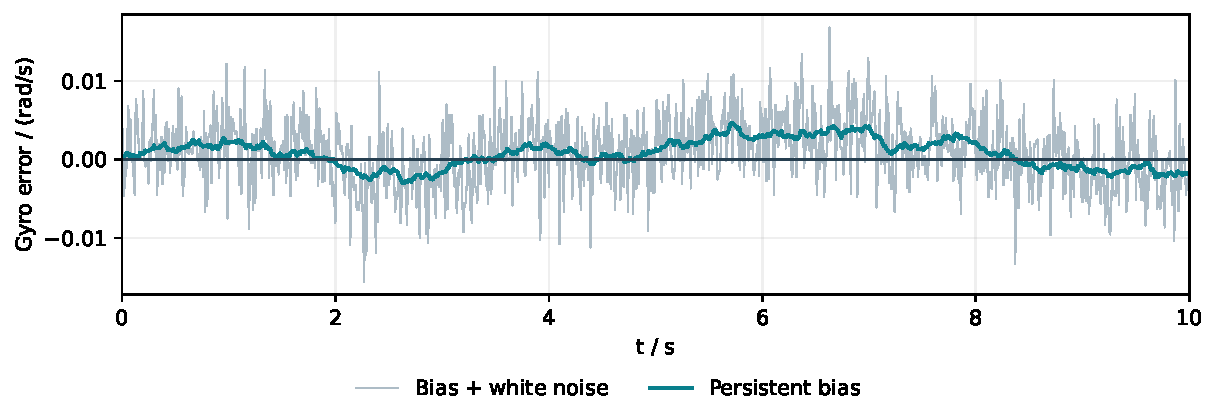
\includegraphics[width=\linewidth]{figures/appC_bias.pdf}
\caption{静止陀螺仪的一个单轴时间序列。深色是累积偏置，浅色在其上叠加每采样 0.004 rad/s 白噪声；短时抖动围绕当前偏置发生。}
\end{minipage}\end{center}
本图适合看误差随时间的形状。要估计“10 秒后偏置有多分散”，则从同一初值重复运行，
每次使用独立增量序列，只取各次的 10 秒终点。

\section{用许多终点估计方差}
记 $M$ 次试验终点为 $z_1,\ldots,z_M$，样本均值与样本方差为
\[
 \bar z=\frac1M\sum_i z_i,\qquad
 s^2=\frac1{M-1}\sum_i(z_i-\bar z)^2.
\]
为什么方差除以 $M-1$？设真实均值为 $\mu$、方差为 $V$。展开平方可得
\[
 \sum_i(z_i-\bar z)^2=\sum_i(z_i-\mu)^2-M(\bar z-\mu)^2.
\]
独立平均的方差为 $\operatorname{Var}(\bar z)=V/M$，两边取期望后右侧为
$MV-M(V/M)=(M-1)V$，所以除以 $M-1$ 后的期望恰为 $V$。
计算时还可展开为
\[
 s^2=\frac{\sum_i z_i^2-M\bar z^2}{M-1},
\]
这就是示例程序中 \code{sum}、\code{square} 和 \code{trials} 的关系。

\begin{center}\begin{minipage}{\linewidth}\makeatletter\def\@captype{figure}\makeatother
\centering
\begin{tikzpicture}[x=1cm,y=1cm,>=stealth,font=\small]
\draw[->,muted] (0,-1.2)--(6.5,-1.2) node[right]{$t$};
\draw[muted,dashed] (5.7,-1.1)--(5.7,1.6);
\draw[thick,tealblue] (0,0)--(1,.2)--(2,.1)--(3,.6)--(4,.4)--(5.7,1.2);
\draw[thick,navy] (0,0)--(1,-.2)--(2,-.1)--(3,-.5)--(4,-.8)--(5.7,-.6);
\draw[thick,orange!80!black] (0,0)--(1,.1)--(2,.3)--(3,.15)--(4,.4)--(5.7,.25);
\foreach \y/\lab in {1.2/z_1,.25/z_2,-.6/z_3}{\fill (5.7,\y) circle (.045) node[right]{$\lab$};}
\fill (0,0) circle (.04) node[left]{$b_0=0$};
\node[below] at (5.7,-1.2){$T$};
\node[anchor=west,align=left] at (7,.4){每次从零开始\\取同一时刻的终点\\计算均值与方差};
\end{tikzpicture}
\caption{独立试验终点的示意。每条折线使用不同增量序列；同一路径上各时刻共享历史，适合研究时间相关性。}
\end{minipage}\end{center}

示例取 $T=10$ s、$\sigma_b=0.002$，100 Hz 与 200 Hz 各运行 5000 次。
程序对每组频率使用固定种子，得到如下终点方差，单位均为 $(\mathrm{rad/s})^2$：
\begin{center}\begin{tabular}{lrr}\toprule
频率 & 理论方差 & 样本方差\\\midrule
100 Hz & $4.0000\times10^{-5}$ & $3.8782\times10^{-5}$\\
200 Hz & $4.0000\times10^{-5}$ & $3.9963\times10^{-5}$\\\bottomrule
\end{tabular}\end{center}
两组应围绕同一个理论值波动；改变频率后每条路径的具体形状可以不同。
将密度加倍，式\eqref{eq:bias_step}使增量加倍、终点方差变为四倍，
这是比观察某一条曲线“是否更抖”更直接的模型检查。

\section{偏置怎样变成角度漂移}
角速度误差积分为角度误差。先考虑固定偏置 $b_0$，则
$e_\psi(T)=\int_0^T b_0\,dt=b_0T$，随时间线性累积。
对于零初值的随机游走，均值仍为零，但角度方差包含各时刻偏置之间的相关性。
把积分看作许多小段相加，再用上一节的协方差公式，有
\begin{align*}
 \operatorname{Var}[e_\psi(T)]
 &=\int_0^T\int_0^T\operatorname{Cov}[b(u),b(v)]\,du\,dv\\
 &=2\sigma_b^2\int_0^T\left(\int_0^v u\,du\right)dv
 =\sigma_b^2\int_0^T v^2\,dv
 =\frac{\sigma_b^2T^3}{3}.
\end{align*}
第二行把正方形积分域分成 $u\le v$ 与 $u\ge v$ 两个对称三角形，前者的最小值为 $u$。
因此角度标准差为 $\sigma_bT^{3/2}/\sqrt3$。取本例参数，10 s 时约为 0.0365 rad。
这是步长趋小时随机游走积分的结果，适合与小步长数值实验比较。

每采样白噪声则按第 06 章给出角度方差 $\sigma_n^2T\Delta t$，因为各项独立。
固定偏置、缓慢偏置变化与独立测量噪声有不同的时间规律，滤波器应分别建模。
第 09 章偏置状态的过程协方差增量 $Q_b=\sigma_b^2\Delta t$ 正对应式\eqref{eq:bias_step}；
估计器还需要借助激光位姿约束，才能从运动观测中修正偏置。
若研究固定\emph{加速度}偏置 $b_a$，则速度误差为 $b_aT$，再次积分得到位置误差
$b_aT^2/2$；此时 $b_a$ 单位为 m/s$^2$，应与陀螺偏置分开计算。

\section{扩展传感器时，先画清时间与坐标}
基础雷达采用单时刻快照，基础 IMU 采用每采样白噪声。
可在独立实验验证后，依次把下面的变化接入传感器与估计接口。

\subsection{延迟改变到达时刻，保留采集时刻}
采集时刻 $t_s$ 的测量描述 $t_s$ 的状态，经过延迟 $\ell$ 后在 $t_a=t_s+\ell$ 到达。
例如一帧激光在 1.00 s 采集，1.08 s 到达；它应校正历史 1.00 s 状态，再按第 09 章缓存重传播。
若把 header 改成 1.08 s，就会把过去环境强行匹配到现在的位姿。
实现时可用按到达时间排序的队列保存消息，内部 header 保持原采集值。
先固定 80 ms 延迟，再增加乱序或丢包，分别观察历史缓存与缺测传播。

\subsection{逐束扫描需要逐束位姿}
旋转扫描中，第 $i$ 束在 $t_i=t_0+i\Delta t_b$ 采集。
设 $T(t_i)$ 把采集时刻的雷达坐标变到固定世界，单束局部点为
$p_i=(r_i\cos\theta_i,r_i\sin\theta_i)$。
先写成世界点 $q=T(t_i)p_i$，再变到选定参考时刻的雷达系：
\[
 p_{\rm ref}=T(t_{\rm ref})^{-1}T(t_i)p_i.
\]
例如雷达朝 x 正向匀速 1 m/s 平移，固定墙在世界 x=5 m。
取两个朝 x 正向的光束，0 s 的束测得 5 m，0.1 s 的束测得 4.9 m。统一到 0 s 时，第二束加回 0.1 m 位移，
两者都落在 5 m 的墙上。
仿真器用各采集时刻的真实状态生成量程，估计器用估计运动完成去畸变；
记录逐束时间后，才有依据区分快照、原始畸变点云和校正后点云。

\subsection{复杂环境会改变哪一层}
凹多边形首先改变几何查询：点是否在内部、圆盘扫掠是否碰撞、射线最近击中哪一条边。
可以画一个 U 形障碍，把凹口中的点作为自由点，再逐项对照这些查询结果。
第 03 章的随机凸多边形可作为基础对照。

动态障碍还增加时间维。例如一个圆心按 $c(t)=(1-t,0)$ 运动，半径 0.2 m；
先取半径为零的质点机器人静止在原点，当前净空为 0.8 m，1 s 后障碍却到达原点。
规划因此要比较对应时刻的机器人与障碍位置，而静态 ESDF 只描述一个时刻的几何。

全局重定位可以从“把机器人移动到远离上次估计的位置”开始实验。
先用当前局部 ICP 初值观察对应点为何匹配失败，再增加分散的候选位姿并逐个几何验证。
把候选搜索、局部优化和候选评分分别记录，有助于判断哪一步限制了恢复范围。

\section{练习：先预测，再用数据核对}
\begin{enumerate}
\item \textbf{代码 appC-1：}补齐随机游走步长；固定 $\xi=1$ 检查 $\Delta t$ 变四倍时增量的变化。
\item 从独立增量推导总方差与两个时刻的协方差；解释为何一条曲线上的样本不能替代独立终点。
\item 展开样本方差公式，手算三个终点 $(-0.01,0,0.01)$ rad/s 的均值与无偏方差。
\item 把密度加倍、总时间加倍，分别预测终点方差与积分角度方差的倍数，再做独立重复实验。
\item 用固定加速度偏置推导位置漂移 $b_aT^2/2$，与陀螺积分的单位逐项比较。
\item 按本章平移墙面例子手算两束去畸变；再设计一个固定延迟实验，标明采集、到达和校正时刻。
\end{enumerate}
练习与扩展实验说明见 \code{exercises/appC/README.md}。
